\documentclass[conference]{IEEEtran}
  \IEEEoverridecommandlockouts

  \usepackage{cite}
  \usepackage{amsmath,amssymb,amsfonts}
  \usepackage{graphicx}
  \usepackage{textcomp}
  \usepackage{xcolor}

  \begin{document}

  \title{{\fontsize{20}{20}\selectfont Cross-Correlation and FFT Phase Analysis for Defect Detection in Active
  Thermography of FRP Composites}}
  \author{
    \IEEEauthorblockN{{\fontsize{12}{11}\selectfont Ayushmaan Puri}}
    \IEEEauthorblockA{
    \textit{{Computer Science and Engineering}}\\
    {University of California, San Diego}\\
    {aypuri@ucsd.edu}
    }
    \and
    \IEEEauthorblockN{{\fontsize{12}{11}\selectfont Dr. Ravibabu Mulaveesala}}
    \IEEEauthorblockA{
    \textit{{InfraRed Imaging Laboratory (IRIL), SeNSE}}\\
    {Indian Institute of Technology, Delhi}\\
    {mulaveesala@sense.iitd.ac.in}
    }
    }

  \maketitle

  \begin{abstract}
  We present a per-pixel signal processing pipeline for detecting subsurface
  defects in fibre-reinforced polymer (FRP) composites using active thermography.
  For each pixel in a recorded thermal video, the temporal intensity signal is
  linearly detrended and then cross-correlated with a reference pixel located in
  a sound (defect-free) region. The central main lobe of the resulting
  cross-correlation is extracted, and the phase of its discrete Fourier transform
  (DFT) is computed. Experiments are conducted on Carbon Fibre-Reinforced Polymer
  (CFRP) specimens under Linear Frequency Modulated (LFM) excitation and Glass
  Fibre-Reinforced Polymer (GFRP) specimens under active pulsed and flux
  excitation. For flux-excited GFRP specimens the FFT phase of the extracted
  correlation window produces clearly distinct spatial signatures that localise
  subsurface defects, while active pulsed excitation is shown to be insufficient
  for phase-based discrimination with this pipeline. The results demonstrate
  the potential of the approach --- and its sensitivity to excitation waveform
  --- for non-destructive evaluation of composite structures.
  \end{abstract}

  \begin{IEEEkeywords}
  active thermography, non-destructive testing, fibre-reinforced polymer,
  cross-correlation, FFT phase, defect detection, LFM excitation
  \end{IEEEkeywords}

  % -----------------------------------------------------------------------
  \section{Introduction}

  Fibre-reinforced polymer (FRP) composites are widely used in aerospace,
  civil, and mechanical engineering due to their high strength-to-weight ratio.
  Subsurface manufacturing defects such as delaminations and voids can
  significantly compromise structural integrity, making non-destructive testing
  (NDT) an essential part of quality assurance.

  Active thermography is an established NDT technique in which an external heat
  source excites the specimen and the resulting surface thermal response is
  recorded by an infrared camera \cite{maldague2001}. Subsurface defects alter
  local heat diffusion, producing surface thermal anomalies that are detectable
  in the recorded video. Among the available excitation strategies, Linear
  Frequency Modulated (LFM) thermal excitation has attracted attention because
  the chirp waveform allows depth resolution to be traded against acquisition
  time \cite{mulaveesala2006}. Infrared thermal wave imaging has been applied
  to FRP composites under a range of such excitation strategies, demonstrating
  effective defect detection in both CFRP and GFRP specimens
  \cite{siddiqui2015,rani2020}.

  A variety of signal processing methods have been applied to thermographic
  sequences, including pulsed phase thermography, thermographic signal
  reconstruction, and principal component analysis. Cross-correlation has also
  been explored as a means of thermally characterising CFRP materials through
  a pulse-compression framework \cite{mulaveesala2011}. In this work, we
  investigate a pipeline that combines per-pixel linear detrending, full
  cross-correlation with a reference signal, main lobe extraction, and DFT
  phase computation. The method is applied to three datasets spanning two
  material systems and two excitation modalities.

  % -----------------------------------------------------------------------
  \section{Experimental Datasets}

  Three thermographic video datasets are used in this study.

  \begin{itemize}
      \item \textbf{CFRP LFM.} A Carbon Fibre-Reinforced Polymer specimen
      excited with a Linear Frequency Modulated thermal stimulus. The video
      has a spatial resolution of $169 \times 289$\,pixels, a frame rate of
      25\,fps, and a total duration of 40\,s ($\approx$1000 frames).

      \item \textbf{GFRP AP.} A Glass Fibre-Reinforced Polymer specimen under
      Active Pulsed excitation, recorded at a spatial resolution of approximately
      $460 \times 460$\,pixels over 1010 frames at 25\,fps.

      \item \textbf{GFRP Flux.} A GFRP specimen under flux excitation, recorded
      at a spatial resolution of approximately $572 \times 458$\,pixels over
      1010 frames at 25\,fps.
  \end{itemize}

  All videos are acquired in greyscale. Fig.~\ref{fig:raw_signal} shows the
  temporal intensity profile of pixel $(200,\,200)$ from the GFRP flux dataset
  over the first 180 of 1010 frames, illustrating two repeating cycles of an
  amplitude-modulated oscillation with increasing intra-cycle frequency,
  consistent with the flux excitation waveform.

  \begin{figure}[t]
      \centering
      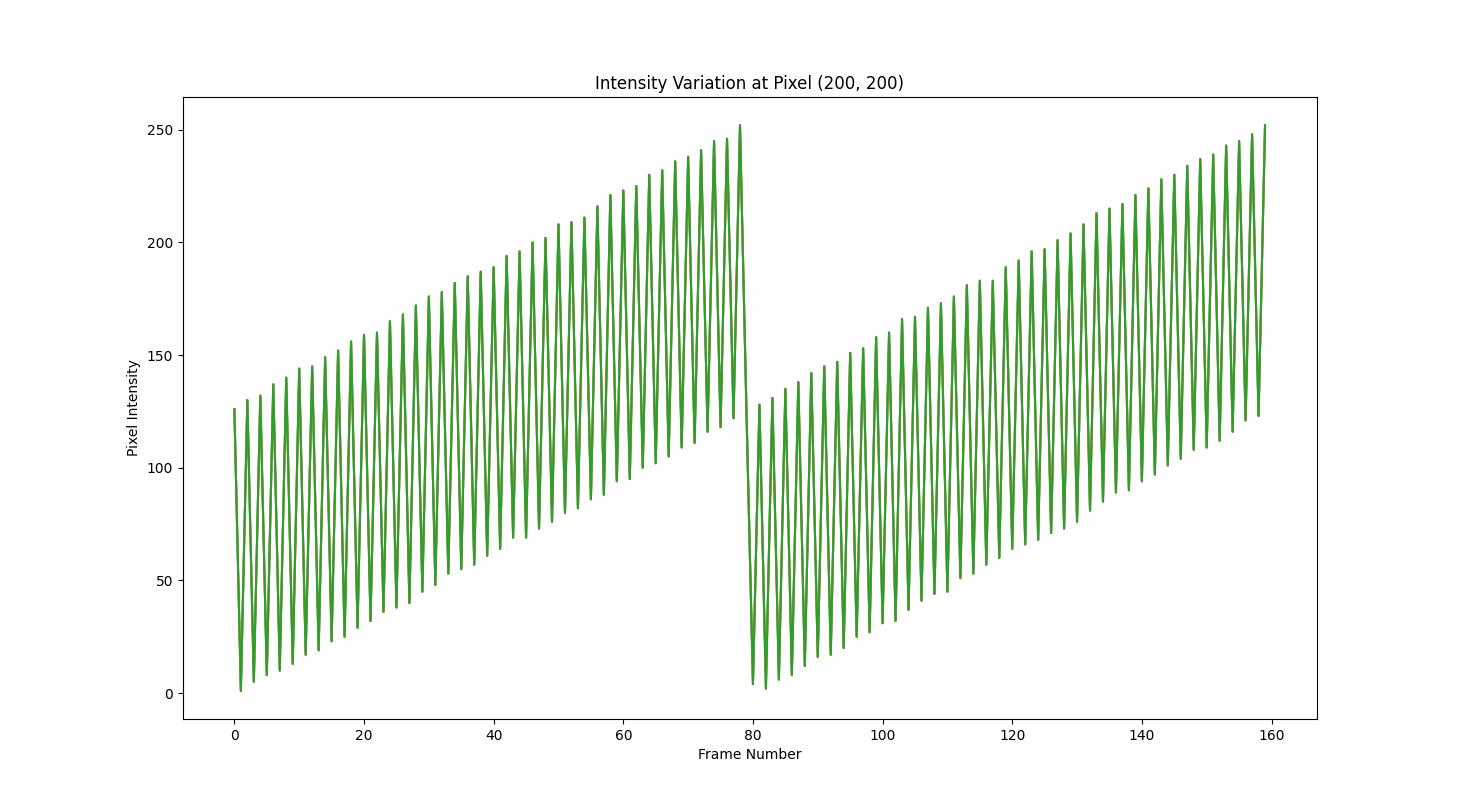
\includegraphics[width=\columnwidth]{figures/gfrp_flux_raw_intensity_pixel_200_200.png}
      \caption{Temporal intensity signal at pixel $(200,\,200)$ in the GFRP flux
      dataset (first 180 of 1010 frames shown). Two repeating cycles of
      increasing-frequency oscillation are visible, consistent with the flux
      excitation waveform.}
      \label{fig:raw_signal}
  \end{figure}

  % -----------------------------------------------------------------------
  \section{Signal Processing Methodology}

  The processing pipeline is applied independently and identically to every
  spatial pixel. Fig.~\ref{fig:single_corr} gives an example of the intermediate
  cross-correlation output.

  \subsection{Greyscale Normalisation}

  Each video frame is converted to greyscale and cast to a 64-bit
  floating-point representation normalised to the range $[0,\,1]$.

  \subsection{Linear Detrending}

  Let $I(x,\,y,\,t)$ denote the normalised intensity of pixel $(x,\,y)$ at
  frame $t$. A linear trend is estimated for each pixel via least-squares
  regression:
  \begin{equation}
      \hat{I}(x,\,y,\,t) \;=\; \alpha\,t + \beta,
  \end{equation}
  with slope $\alpha$ and intercept $\beta$ fit to the full temporal sequence.
  The detrended signal is
  \begin{equation}
      \tilde{I}(x,\,y,\,t) \;=\; I(x,\,y,\,t) - \hat{I}(x,\,y,\,t).
  \end{equation}
  This step removes slow bulk-heating drift, leaving the thermally-driven
  response to the excitation waveform.

  \subsection{Cross-Correlation with a Reference Pixel}

  Each detrended signal $\tilde{I}(x,\,y,\,\cdot)$ is cross-correlated with the
  signal at a designated reference pixel $(x_0,\,y_0)$ located in a
  sound region:
  \begin{equation}
      R_{xy}(\tau) \;=\; \sum_{t=0}^{N-1}\,
      \tilde{I}(x,\,y,\,t)\;\tilde{I}(x_0,\,y_0,\,t - \tau),
  \end{equation}
  where samples outside $[0,\,N-1]$ are treated as zero (zero-extension).
  The full cross-correlation is computed using \texttt{numpy.correlate} in
  \texttt{full} mode (GFRP AP, GFRP flux) or \texttt{same} mode (CFRP LFM),
  yielding an output of length $2N-1$ or $N$ respectively. The \texttt{same}
  mode was used for the CFRP LFM dataset to match the output length to the
  input signal length; \texttt{full} mode was used for the GFRP datasets to
  retain all lag values. No coefficient normalisation is applied; raw
  cross-correlation values are retained.
  For the CFRP LFM, GFRP AP, and GFRP flux datasets the reference pixel is
  located at coordinates $(100,\,100)$, $(200,\,200)$, and $(200,\,200)$
  respectively, all chosen from visually defect-free regions of the specimen.
  This approach is related to the pulse-compression framework applied to
  CFRP characterisation in \cite{mulaveesala2011}, but operates directly on
  a per-pixel reference signal rather than a synthetic matched filter.

  \subsection{Correlation Window Extraction}

  A fixed temporal window of the cross-correlation is extracted for further
  analysis. Both GFRP datasets comprise 1010 frames, giving a full-mode
  correlation output of $2\times1010-1=2019$ frames with the zero-lag peak
  at index~1009. The GFRP flux window (frames 930--1090, 160 frames) is
  centred on this zero-lag peak and constitutes the main lobe extraction.
  For the CFRP LFM dataset ($N=1001$, \texttt{same} mode, output length 1001)
  the zero-lag peak falls at index~500; a 10-frame window (frames 430--440,
  centred at index~435, approximately 65 samples before zero-lag) was selected
  by inspection of single-pixel correlation traces. For the GFRP AP dataset the window spans
  frames 400--610 (210 frames of the 2019-frame output, centred at index~505),
  which lies approximately 500 samples before the zero-lag peak at index~1009;
  this off-centre placement reflects the empirical response structure of the
  active-pulsed excitation and is consistent with the negative phase-separation
  result discussed in Section~IV.

  \subsection{FFT Phase Computation}

  The discrete Fourier transform is applied to the extracted correlation window,
  and its phase spectrum is retained:
  \begin{equation}
      \phi_{xy}(k) \;=\; \angle\;\mathcal{F}\!\left\{R_{xy}(\tau)\right\}[k],
  \end{equation}
  where $k$ indexes frequency bin. This per-pixel phase sequence constitutes
  the primary output used for defect discrimination.

  \subsection{Discretisation (Zero-Padding)}

  To investigate the effect of frequency resolution on the phase output, the
  detrended signals are zero-padded to $N_d$ samples prior to correlation.
  For the GFRP AP dataset, $N_d \in \{210,\,420,\,630,\,840,\,1000,\,2048,\,4096\}$
  is explored. For the GFRP flux dataset,
  $N_d \in \{160,\,640,\,1024,\,2048\}$ is used.

  % -----------------------------------------------------------------------
  \section{Results}

  \subsection{Cross-Correlation}

  Fig.~\ref{fig:single_corr} shows the cross-correlation of pixel
  $(70,\,190)$ with the reference in the CFRP LFM dataset. A well-defined
  main lobe is visible at the centre of the correlation, flanked by decaying
  side lobes characteristic of an LFM waveform.

  \begin{figure}[t]
      \centering
      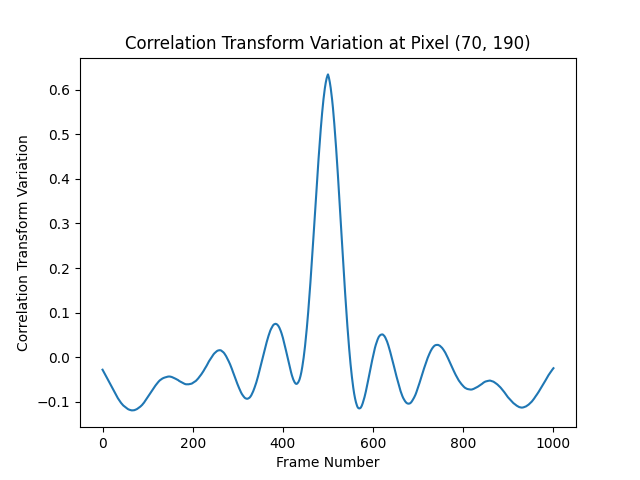
\includegraphics[width=\columnwidth]{figures/cfrp_lfm_corr_pixel_70_190.png}
      \caption{Cross-correlation of pixel $(70,\,190)$ with the reference pixel
      in the CFRP LFM dataset. A distinct main lobe is centred at zero lag,
      with decaying side lobes on either side.}
      \label{fig:single_corr}
  \end{figure}

  Fig.~\ref{fig:defect_vs_sound} compares the cross-correlation signals for
  twelve defect pixels against a sound reference pixel in the GFRP flux dataset.
  While most defect pixels exhibit broadly similar main-lobe shapes, several
  show elevated pre-peak side-lobe energy and asymmetric lobe structure compared
  to the sound pixel, consistent with altered heat diffusion over subsurface
  anomalies.

  \begin{figure}[t]
      \centering
      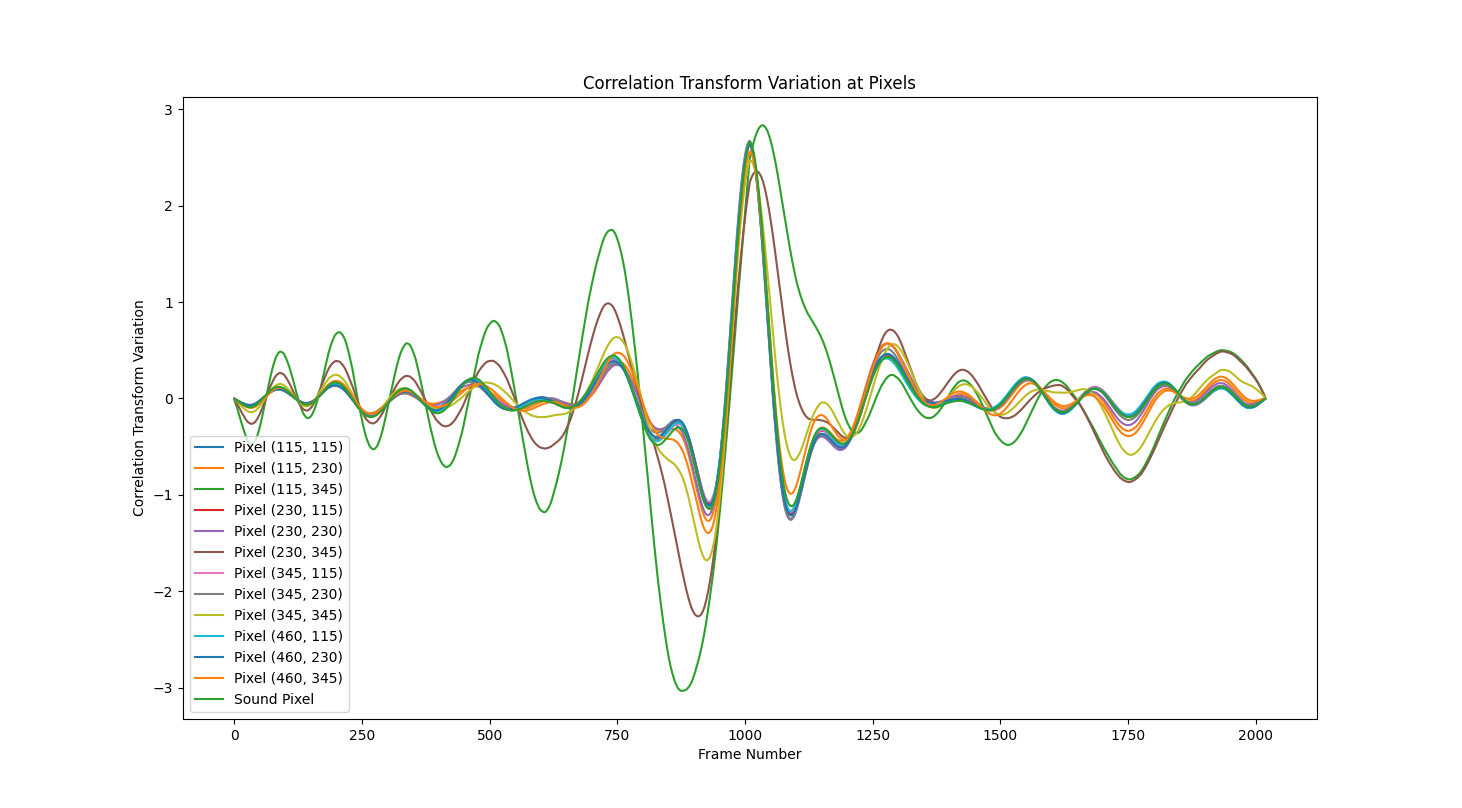
\includegraphics[width=\columnwidth]{figures/gfrp_flux_corr_defect_vs_sound_12pixel.png}
      \caption{Cross-correlation signals for twelve defect pixels and one sound
      pixel in the GFRP flux dataset. Some defect pixels display elevated
      pre-peak side lobes not present in the sound pixel.}
      \label{fig:defect_vs_sound}
  \end{figure}

  Fig.~\ref{fig:gfrp_ap_phase} shows the FFT phase of the correlation window
  for two defect pixels and one sound pixel in the GFRP AP dataset.
  All three profiles are nearly indistinguishable: each exhibits a sharp
  peak near $+\pi$ at bin~1, decays sharply to approximately $-2.5$\,rad
  at bin~2, and then rises smoothly toward zero across the remaining bins.
  The absence of phase separation between defect and sound pixels indicates
  that the active pulsed excitation does not imprint a frequency-localised
  phase signature in the extracted correlation window, in contrast to the
  results obtained with flux excitation below.

  \begin{figure}[t]
      \centering
      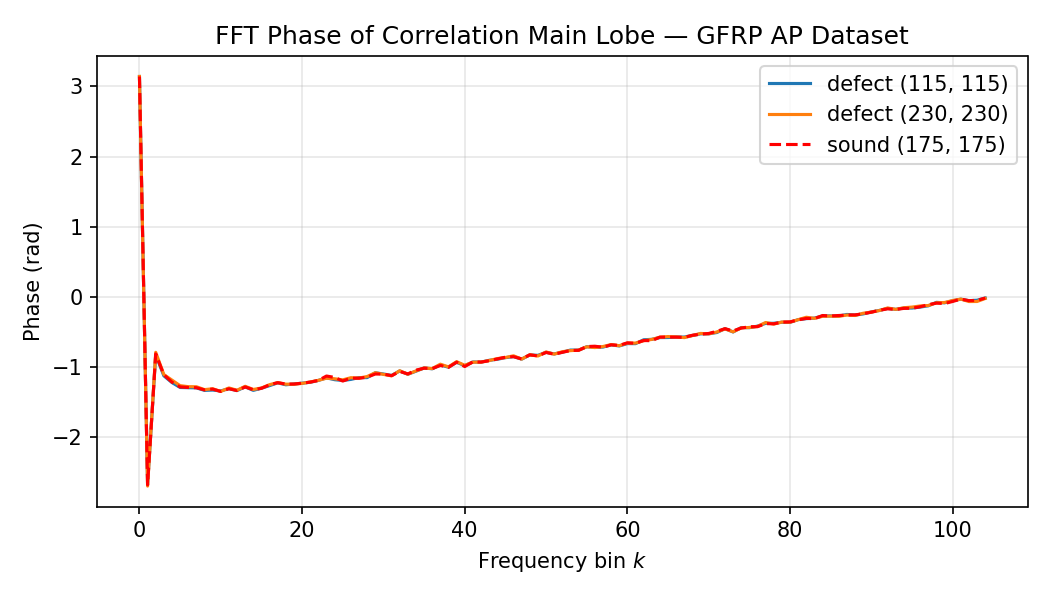
\includegraphics[width=\columnwidth]{figures/gfrp_ap_fft_phase_defect_vs_sound.png}
      \caption{FFT phase of the extracted correlation window for two defect
      pixels --- $(115,\,115)$ and $(230,\,230)$ --- and the sound pixel at
      $(175,\,175)$ in the GFRP AP dataset. All three profiles overlap,
      indicating that active pulsed excitation does not produce
      phase-separated signatures with this pipeline.}
      \label{fig:gfrp_ap_phase}
  \end{figure}

  \subsection{FFT Phase of the Correlation Main Lobe}

  Fig.~\ref{fig:fft_phase} shows the FFT phase of the main lobe for three
  defect pixels and one sound pixel in the GFRP flux dataset. Two of the defect
  pixels --- at $(115,\,230)$ and $(115,\,345)$ --- produce nearly identical phase
  profiles: the phase rapidly saturates near $+\pi$, then drops discontinuously
  to $-\pi$ around frequency bin~80 before decaying. The third defect pixel at
  $(115,\,115)$ exhibits a markedly slower, quasi-linear phase sweep across the
  full 160-bin range with a single wrap discontinuity. In contrast, the sound
  pixel at $(10,\,10)$ shows high-frequency oscillations of large amplitude
  throughout, with no structured sweep. The three qualitatively distinct
  behaviours --- fast-saturating, slow-sweeping, and rapidly oscillating ---
  demonstrate that the FFT phase of the correlation main lobe separates material
  regions according to their thermophysical character.

  \begin{figure}[t]
      \centering
      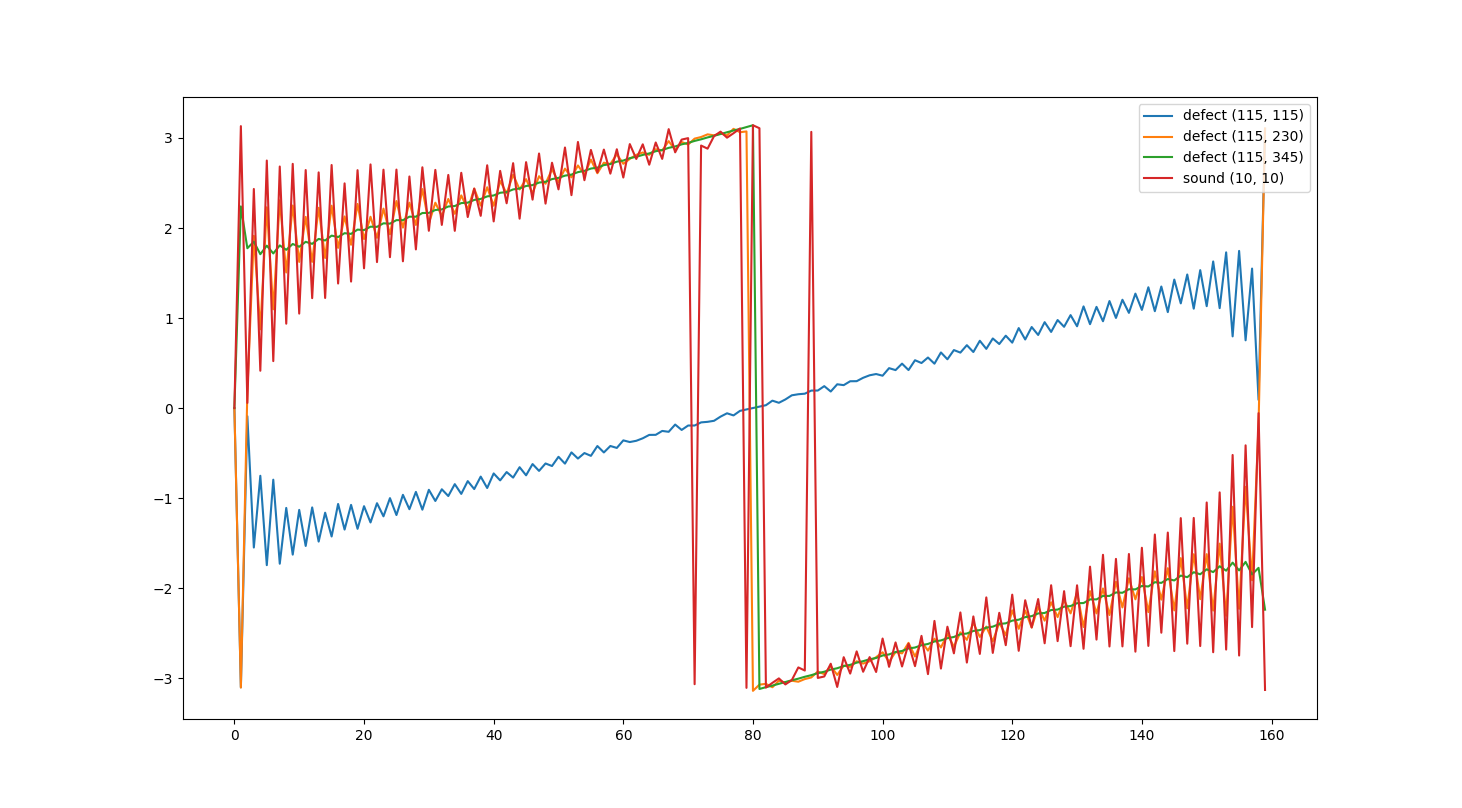
\includegraphics[width=\columnwidth]{figures/gfrp_flux_fft_phase_corr_mainlobe_defect_vs_sound.png}
      \caption{FFT phase of the correlation main lobe for three defect pixels and
      one sound pixel in the GFRP flux dataset. Defect pixels at $(115,\,230)$
      and $(115,\,345)$ (orange and green) share a fast-saturating profile;
      $(115,\,115)$ (blue) exhibits a slow quasi-linear sweep; the sound pixel
      $(10,\,10)$ (red) oscillates rapidly with no structured variation.}
      \label{fig:fft_phase}
  \end{figure}

  \subsection{Spatial Phase Map}

  Fig.~\ref{fig:phase_map} renders the per-pixel FFT phase at frequency
  bin~10 as a 2D spatial image for the GFRP flux dataset. Bin~10 was
  selected as the frequency index at which defect-to-sound phase contrast
  was visually maximised across the spatial map. Six to eight circular
  regions of elevated phase are clearly visible, arranged in a regular grid
  pattern consistent with the known subsurface defect layout of the specimen.
  The surrounding sound material produces a distinct, spatially uniform phase
  level. Phase values were mapped to the range $[0,\,255]$ for video storage
  prior to display, so the colorbar reflects this normalised scale rather than
  absolute radians. This demonstrates that the pipeline generates spatially
  resolved defect maps directly from the per-pixel phase computation, without
  any segmentation or post-processing step.

  \begin{figure}[t]
      \centering
      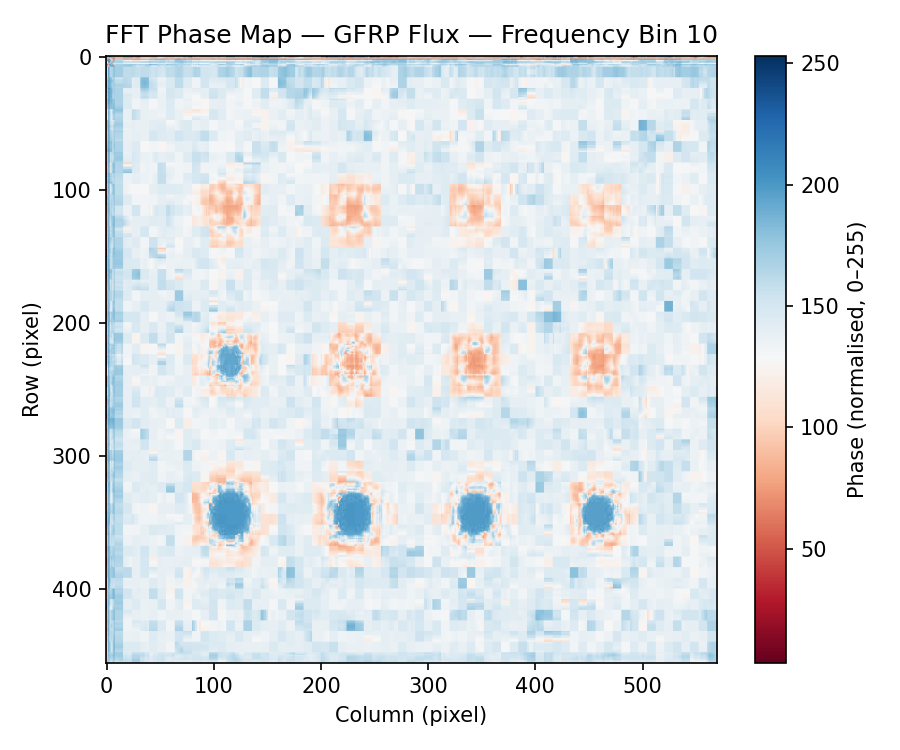
\includegraphics[width=\columnwidth]{figures/gfrp_flux_phase_map_bin10.png}
      \caption{Spatial FFT phase map at frequency bin~10 for the GFRP flux
      dataset. Circular anomalous regions (defects) are clearly separated from
      the surrounding sound material, demonstrating per-pixel spatial
      resolution of the pipeline.}
      \label{fig:phase_map}
  \end{figure}

  \subsection{Discretisation Sensitivity}

  Fig.~\ref{fig:disc_sensitivity} shows the FFT phase of defect pixel
  $(115,\,230)$ at zero-padding levels $N_d \in \{160,\,640,\,1024\}$ for
  the GFRP flux dataset. Phase values are read from the per-$N_d$ output
  videos (normalised to $[0,\,255]$ for storage), so the $y$-axis reflects
  this normalised scale. All three profiles exhibit the same oscillatory
  structure across the normalised frequency range; increasing $N_d$ provides
  finer frequency resolution but does not alter the qualitative shape of the
  phase profile. This confirms that the discriminating features are stable
  across a wide range of padding choices, and that $N_d = 160$ (the natural
  main lobe length) already captures the essential phase behaviour.

  \begin{figure}[t]
      \centering
      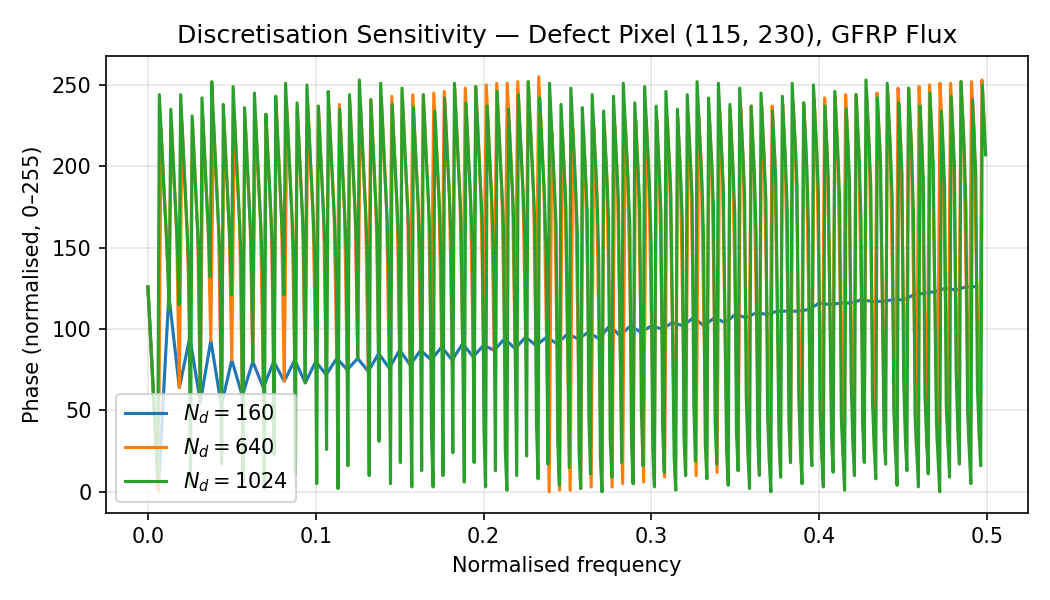
\includegraphics[width=\columnwidth]{figures/gfrp_flux_disc_sensitivity.png}
      \caption{FFT phase of defect pixel $(115,\,230)$ in the GFRP flux
      dataset at three zero-padding levels. Increasing $N_d$ refines frequency
      resolution but leaves the qualitative phase profile unchanged.}
      \label{fig:disc_sensitivity}
  \end{figure}

  % -----------------------------------------------------------------------
  \section{Discussion}

  Linear detrending effectively removes bulk-heating drift, leaving the
  excitation-driven component of each pixel's thermal signal. Cross-correlation
  then measures the similarity of this component to the reference pixel's
  response as a function of temporal lag, enhancing defect contrast by
  suppressing spatially uniform background.

  The FFT phase computed over the main lobe provides a frequency-domain
  signature that is qualitatively distinct between defective and sound regions
  in the GFRP flux dataset. The slow quasi-linear phase sweep observed for pixel
  $(115,\,115)$ and the fast-saturating profiles of $(115,\,230)$ and
  $(115,\,345)$ suggest that defects at different locations --- and potentially
  different depths --- produce different phase responses. The rapidly oscillating
  phase of the sound pixel, by contrast, carries no structured trend. This
  structured vs.\ unstructured phase behaviour is the key discriminating
  observable, and the spatial phase map (Fig.~\ref{fig:phase_map}) shows that it
  generalises across the specimen surface with sub-region spatial resolution.

  The absence of phase separation in the GFRP AP dataset
  (Fig.~\ref{fig:gfrp_ap_phase}) reflects the waveform structure of active
  pulsed excitation. A short broadband thermal pulse produces a diffuse thermal
  response in which defect-induced diffusivity differences manifest as small
  amplitude perturbations rather than frequency-localised phase shifts. The
  cross-correlation of two such pulse responses resembles an autocorrelation of
  a broad impulse response function, which is symmetric and concentrated at
  zero lag regardless of local diffusivity. As a result, the phase of the
  correlation window is dominated by the excitation waveform rather than
  material properties, preventing defect discrimination. Chirp-based (LFM) and
  flux-based excitations sweep frequency over time and therefore impart
  structured time-frequency content; this is what enables the per-frequency
  phase diversity exploited by the pipeline.

  The discretisation experiments (Fig.~\ref{fig:disc_sensitivity}) confirm that
  the qualitative phase profile is stable across a wide range of zero-padding
  levels, so practitioners can choose $N_d$ for computational convenience
  without sacrificing discriminating power. A systematic quantitative analysis
  relating disc level $N_d$ to defect depth is left for future work, building
  on depth-resolved pulse compression approaches developed for GFRP
  characterisation \cite{rani2020}.

  % -----------------------------------------------------------------------
  \section{Conclusion}

  We have presented and evaluated a signal processing pipeline for active
  thermographic NDT of FRP composites. The pipeline --- linear detrending,
  full cross-correlation with a sound reference pixel, main lobe extraction,
  and FFT phase computation --- is applied to CFRP (LFM excitation) and GFRP
  (active pulsed and flux excitation) datasets \cite{siddiqui2015}. For the
  GFRP flux dataset the FFT phase of the correlation main lobe produces
  qualitatively distinct signatures that clearly separate defective from
  healthy material regions and, when rendered as a 2D spatial map, reveals
  the subsurface defect layout without additional segmentation. The pipeline's
  discriminating power is sensitive to excitation waveform: active pulsed
  excitation does not produce phase separation, whereas the GFRP flux dataset
  --- which carries structured time-frequency content --- does. The CFRP LFM
  cross-correlation displays expected main-lobe structure consistent with
  chirp-based excitation; per-pixel phase discrimination for that dataset is
  reserved for future work. Future work will establish quantitative relationships
  between the phase profile shape and defect depth, and will investigate
  adaptive reference-pixel selection to improve robustness.

  % -----------------------------------------------------------------------
  \begin{thebibliography}{1}

  \bibitem{maldague2001}
  X.~Maldague,
  \textit{Theory and Practice of Infrared Technology for Nondestructive Testing}.
  Wiley-Interscience, New York, 2001.

  \bibitem{mulaveesala2006}
  R.~Mulaveesala and S.~Tuli,
  ``Theory of frequency modulated thermal wave imaging for nondestructive
  subsurface defect detection,''
  \textit{Applied Physics Letters}, vol.~89, no.~19, p.~191913, 2006.

  \bibitem{siddiqui2015}
  J.~A.~Siddiqui, V.~Arora, R.~Mulaveesala, and A.~Muniyappa,
  ``Infrared thermal wave imaging for nondestructive testing of
  fibre reinforced polymers,''
  \textit{Experimental Mechanics},
  vol.~55, pp.~1239--1245, 2015.

  \bibitem{rani2020}
  A.~Rani and R.~Mulaveesala,
  ``Depth resolved pulse compression favourable frequency modulated
  thermal wave imaging for quantitative characterization of glass
  fibre reinforced polymer,''
  \textit{Infrared Physics \& Technology},
  vol.~110, p.~103441, 2020.

  \bibitem{mulaveesala2011}
  R.~Mulaveesala and V.~S.~Ghali,
  ``Cross-correlation-based approach for thermal non-destructive
  characterisation of carbon fibre reinforced plastics,''
  \textit{Insight -- Non-Destructive Testing and Condition Monitoring},
  vol.~53, no.~1, pp.~34--36, Jan. 2011.

  \end{thebibliography}

  \end{document}